\documentclass[10pt,letterpaper]{article}

\usepackage[margin=0.75in]{geometry}
\usepackage{tikz}
\usepackage{amsmath}
\begin{document}

  \title{CS 321, Assignment 6}
  \author{Cody Malick\\
  \texttt{malickc@oregonstate.edu}}
  \date{\today}
  \maketitle

\section{}
\subsection*{a}
Given some machine $M=\{Q,\Sigma,\delta,s,F\}$ and a CFG 
$G=\{A_p \rightarrow cA_q | \delta(p,c)\} 
\cup \{A_p \rightarrow \epsilon | p \in F\}$\\\\

$\delta^*(s,w) = q \iff A_s \overset{*}{\iff} wA_q$\\\\

\noindent Base Case:\\
$w=\epsilon, q=q\\
A_s \overset{*}{\iff} A_s = \epsilon A_s$\\\\

\noindent Inductive Step:\\
$w = xb$, assuming the inductive hypothesis is true for x.\\
$\delta^*(s,xb)=\delta(\delta^*(s,x),b)$\\
$p=\delta^*(s,x)$\\
$q=\delta(p,b) \iff A_p \Rightarrow bA_q$\\
$\delta^*(s,x) = p \iff A_s \Rightarrow xA_p=A_s \Rightarrow x(bA_q) = A_s \Rightarrow wA_q$

Because $p = \delta^*(s,x)$ then we can show that reading an additional
character is no different than reading a character in the original string.

Therefore, the inductive hypothesis holds. 

\subsection*{b}
Original: \\

\begin{center}
	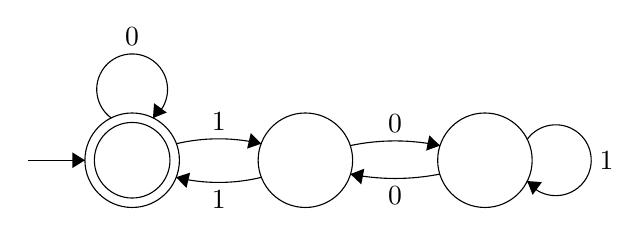
\begin{tikzpicture}[scale=0.2]
		\tikzstyle{every node}+=[inner sep=0pt]
		\draw [black] (12.4,-10.8) circle (3);
		\draw [black] (12.4,-10.8) circle (2.4);
		\draw [black] (23.4,-10.8) circle (3);
		\draw [black] (34.8,-10.8) circle (3);
		\draw [black] (5.8,-10.8) -- (9.4,-10.8);
		\fill [black] (9.4,-10.8) -- (8.6,-10.3) -- (8.6,-11.3);
		\draw [black] (15.202,-9.752) arc (103.22544:76.77456:11.792);
		\fill [black] (20.6,-9.75) -- (19.93,-9.08) -- (19.7,-10.06);
		\draw (17.9,-8.94) node [above] {$1$};
		\draw [black] (26.246,-9.87) arc (101.89414:78.10586:13.848);
		\fill [black] (31.95,-9.87) -- (31.27,-9.22) -- (31.07,-10.19);
		\draw (29.1,-9.07) node [above] {$0$};
		\draw [black] (31.937,-11.68) arc (-78.79986:-101.20014:14.608);
		\fill [black] (26.26,-11.68) -- (26.95,-12.33) -- (27.14,-11.34);
		\draw (29.1,-12.46) node [below] {$0$};
		\draw [black] (20.612,-11.884) arc (-76.26827:-103.73173:11.425);
		\fill [black] (15.19,-11.88) -- (15.85,-12.56) -- (16.08,-11.59);
		\draw (17.9,-12.71) node [below] {$1$};
		\draw [black] (37.48,-9.477) arc (144:-144:2.25);
		\draw (42.05,-10.8) node [right] {$1$};
		\fill [black] (37.48,-12.12) -- (37.83,-13) -- (38.42,-12.19);
		\draw [black] (11.077,-8.12) arc (234:-54:2.25);
		\draw (12.4,-3.55) node [above] {$0$};
		\fill [black] (13.72,-8.12) -- (14.6,-7.77) -- (13.79,-7.18);
	\end{tikzpicture}
\end{center}


\noindent CFG:\\
$S \rightarrow 0S | 1T | \epsilon$\\
$T \rightarrow 1S | 0U$\\
$U \rightarrow 0T | 1U$\\

\section{}
Starting state:\\
$S \rightarrow aSddd\ |\ T$\\
$T \rightarrow bTdd\ |\ R$\\
$R \rightarrow cR\ |\ \epsilon$\\

Step 1, add new start symbol $S^*$, add rule $S^* \rightarrow S$\\
$S^* \rightarrow S$\\
$S \rightarrow aSddd\ |\ T$\\
$T \rightarrow bTdd\ |\ R$\\
$R \rightarrow cR\ |\ \epsilon$\\

Step 2, Shorten RHS rules for each rule $A \rightarrow \alpha_1, \alpha_2,...,\alpha_k$
where $k \geq 3$\\
$S^* \rightarrow S$\\
$S \rightarrow MN\ |\ T$\\
$M \rightarrow aS$\\
$N \rightarrow dO$\\
$O \rightarrow dd$\\
$T \rightarrow PO\ |\ R$\\
$P \rightarrow bT$\\
$R \rightarrow cR\ |\ \epsilon$\\

Step 3, Clean up mixed RHS\\
$S^* \rightarrow S$\\
$S \rightarrow MN\ |\ T$\\
$M \rightarrow AS$\\
$N \rightarrow DO$\\
$O \rightarrow DD$\\
$T \rightarrow PO\ |\ R$\\
$P \rightarrow BT$\\
$R \rightarrow CR\ |\ \epsilon$\\
$A \rightarrow a$\\
$B \rightarrow b$\\
$C \rightarrow c$\\

Step 4, determine which nonterminal are "nullable" $(A \Rightarrow^* \epsilon)$\\
The only rule that goes to $\epsilon$ is R, so:\\
$S^* \rightarrow S$\\
$S \rightarrow MN\ |\ T$\\
$M \rightarrow AS$\\
$N \rightarrow DO$\\
$O \rightarrow DD$\\
$T \rightarrow PO\ |\ C$\\
$P \rightarrow BT$\\
$A \rightarrow a$\\
$B \rightarrow b$\\
$C \rightarrow c$\\

Step 5, for each rule $A \rightarrow B$, copy all $B \rightarrow \alpha$ rules to
$A \rightarrow \alpha$. Repeat until no more changes, then delete $A \rightarrow B$\\
$S^* \rightarrow MN\ |\ T$\\
$M \rightarrow AS$\\
$N \rightarrow DO$\\
$O \rightarrow DD$\\
$T \rightarrow PO\ |\ c$\\
$P \rightarrow BT$\\
$A \rightarrow a$\\
$B \rightarrow b$\\
$C \rightarrow c$\\

\section{}
\subsection*{a}
$L=\{a^kb^mc^n\ |\ k,m,n not all equal\}$\\
We can solve this problem by building a CFG to show that it's context free:\\
$S \rightarrow\;T \;| \;U \;| \;V \;| \;W \;$\\
$T \rightarrow\;aTbC \;| \;aT \;| \;a$\\ % a > b
$U \rightarrow\;aUBc \;| \;aU \;| \;a$\\ % a > c
$V \rightarrow \;aVbC \;| \;Vb \;| \;b$\\ % b > a
$W \rightarrow \;AbWc \;| \;Wb \;| \;b$\\ % b > c
$A \rightarrow \;aA \;| \;a \;| \;\epsilon$ \\
$B \rightarrow \;Bb \;| \;b \;|\; \epsilon$ \\
$C \rightarrow \;Cc \;| \;c \;| \;\epsilon$ \\
In the above rules, T covers the $a > b$ case, U covers the $a > b$ case, V
covers the $b > a$ case, and W covers the $b > c$ case. We don't need to cover
more cases than this, because with the above rules, one letter will always not
be equal to the others.

\subsection*{b}
We can show that this language is context free by building a pushdown automaton
. The automaton below reads in a set of characters, and for every character
read in before the 'c' character, we push to the stack. These are the characters
in x. After the 'c' char, we read the characters in y. To do this, we
read an arbitrary number of characters, then we read the $rev(x)$ substring
and pop the stack until it's empty. Once it's empty, we read an arbitrary number of
characters again. By using the stack, we can reverse the substring, giving us
$rev(x)$.
\begin{center}
	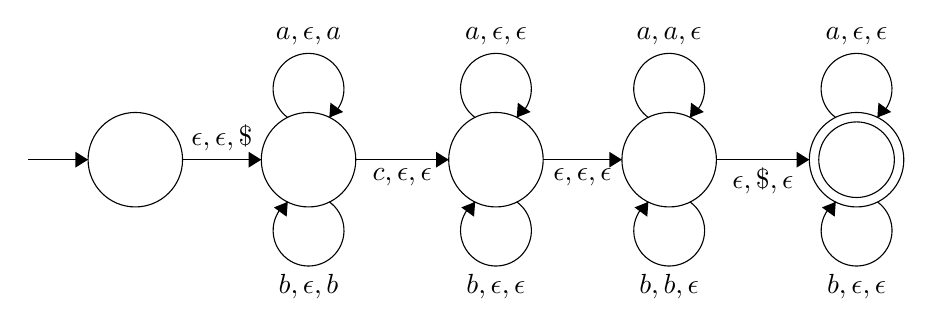
\begin{tikzpicture}[scale=0.2]
		\tikzstyle{every node}+=[inner sep=0pt]
		\draw [black] (11.3,-12.8) circle (3);
		\draw [black] (22.3,-12.8) circle (3);
		\draw [black] (34.2,-12.8) circle (3);
		\draw [black] (45.2,-12.8) circle (3);
		\draw [black] (57.1,-12.8) circle (3);
		\draw [black] (57.1,-12.8) circle (2.4);
		\draw [black] (4.5,-12.8) -- (8.3,-12.8);
		\fill [black] (8.3,-12.8) -- (7.5,-12.3) -- (7.5,-13.3);
		\draw [black] (14.3,-12.8) -- (19.3,-12.8);
		\fill [black] (19.3,-12.8) -- (18.5,-12.3) -- (18.5,-13.3);
		\draw (16.8,-12.3) node [above] {$\epsilon,\epsilon,\$$};
		\draw [black] (20.977,-10.12) arc (234:-54:2.25);
		\draw (22.3,-5.55) node [above] {$a,\epsilon,a$};
		\fill [black] (23.62,-10.12) -- (24.5,-9.77) -- (23.69,-9.18);
		\draw [black] (23.623,-15.48) arc (54:-234:2.25);
		\draw (22.3,-20.05) node [below] {$b,\epsilon,b$};
		\fill [black] (20.98,-15.48) -- (20.1,-15.83) -- (20.91,-16.42);
		\draw [black] (25.3,-12.8) -- (31.2,-12.8);
		\fill [black] (31.2,-12.8) -- (30.4,-12.3) -- (30.4,-13.3);
		\draw (28.25,-13.3) node [below] {$c,\epsilon,\epsilon$};
		\draw [black] (37.2,-12.8) -- (42.2,-12.8);
		\fill [black] (42.2,-12.8) -- (41.4,-12.3) -- (41.4,-13.3);
		\draw (39.7,-13.3) node [below] {$\epsilon,\epsilon,\epsilon$};
		\draw [black] (32.877,-10.12) arc (234:-54:2.25);
		\draw (34.2,-5.55) node [above] {$a,\epsilon,\epsilon$};
		\fill [black] (35.52,-10.12) -- (36.4,-9.77) -- (35.59,-9.18);
		\draw [black] (35.523,-15.48) arc (54:-234:2.25);
		\draw (34.2,-20.05) node [below] {$b,\epsilon,\epsilon$};
		\fill [black] (32.88,-15.48) -- (32,-15.83) -- (32.81,-16.42);
		\draw [black] (43.877,-10.12) arc (234:-54:2.25);
		\draw (45.2,-5.55) node [above] {$a,a,\epsilon$};
		\fill [black] (46.52,-10.12) -- (47.4,-9.77) -- (46.59,-9.18);
		\draw [black] (46.523,-15.48) arc (54:-234:2.25);
		\draw (45.2,-20.05) node [below] {$b,b,\epsilon$};
		\fill [black] (43.88,-15.48) -- (43,-15.83) -- (43.81,-16.42);
		\draw [black] (48.2,-12.8) -- (54.1,-12.8);
		\fill [black] (54.1,-12.8) -- (53.3,-12.3) -- (53.3,-13.3);
		\draw (51.15,-13.3) node [below] {$\epsilon,\$,\epsilon$};
		\draw [black] (55.777,-10.12) arc (234:-54:2.25);
		\draw (57.1,-5.55) node [above] {$a,\epsilon,\epsilon$};
		\fill [black] (58.42,-10.12) -- (59.3,-9.77) -- (58.49,-9.18);
		\draw [black] (58.423,-15.48) arc (54:-234:2.25);
		\draw (57.1,-20.05) node [below] {$b,\epsilon,\epsilon$};
		\fill [black] (55.78,-15.48) -- (54.9,-15.83) -- (55.71,-16.42);
	\end{tikzpicture}
\end{center}

\end{document}
